\documentclass[a4paper,12pt]{article}


\usepackage{graphicx}
\usepackage{tikz}
\usetikzlibrary{positioning, arrows.meta}
\usepackage{amsmath}   
\usepackage{caption}       
\usepackage{xepersian}
\usepackage{setspace}
\usepackage{perpage}
\MakePerPage{footnote}
\usepackage{multirow}



\renewcommand{\contentsname}{فهرست مطالب\\}
\numberwithin{figure}{subsection}
\settextfont[Extension=.ttf]{IRNazanin}

\begin{document}

\begin{titlepage}

    \centering
   \vspace*{-3cm}
    
    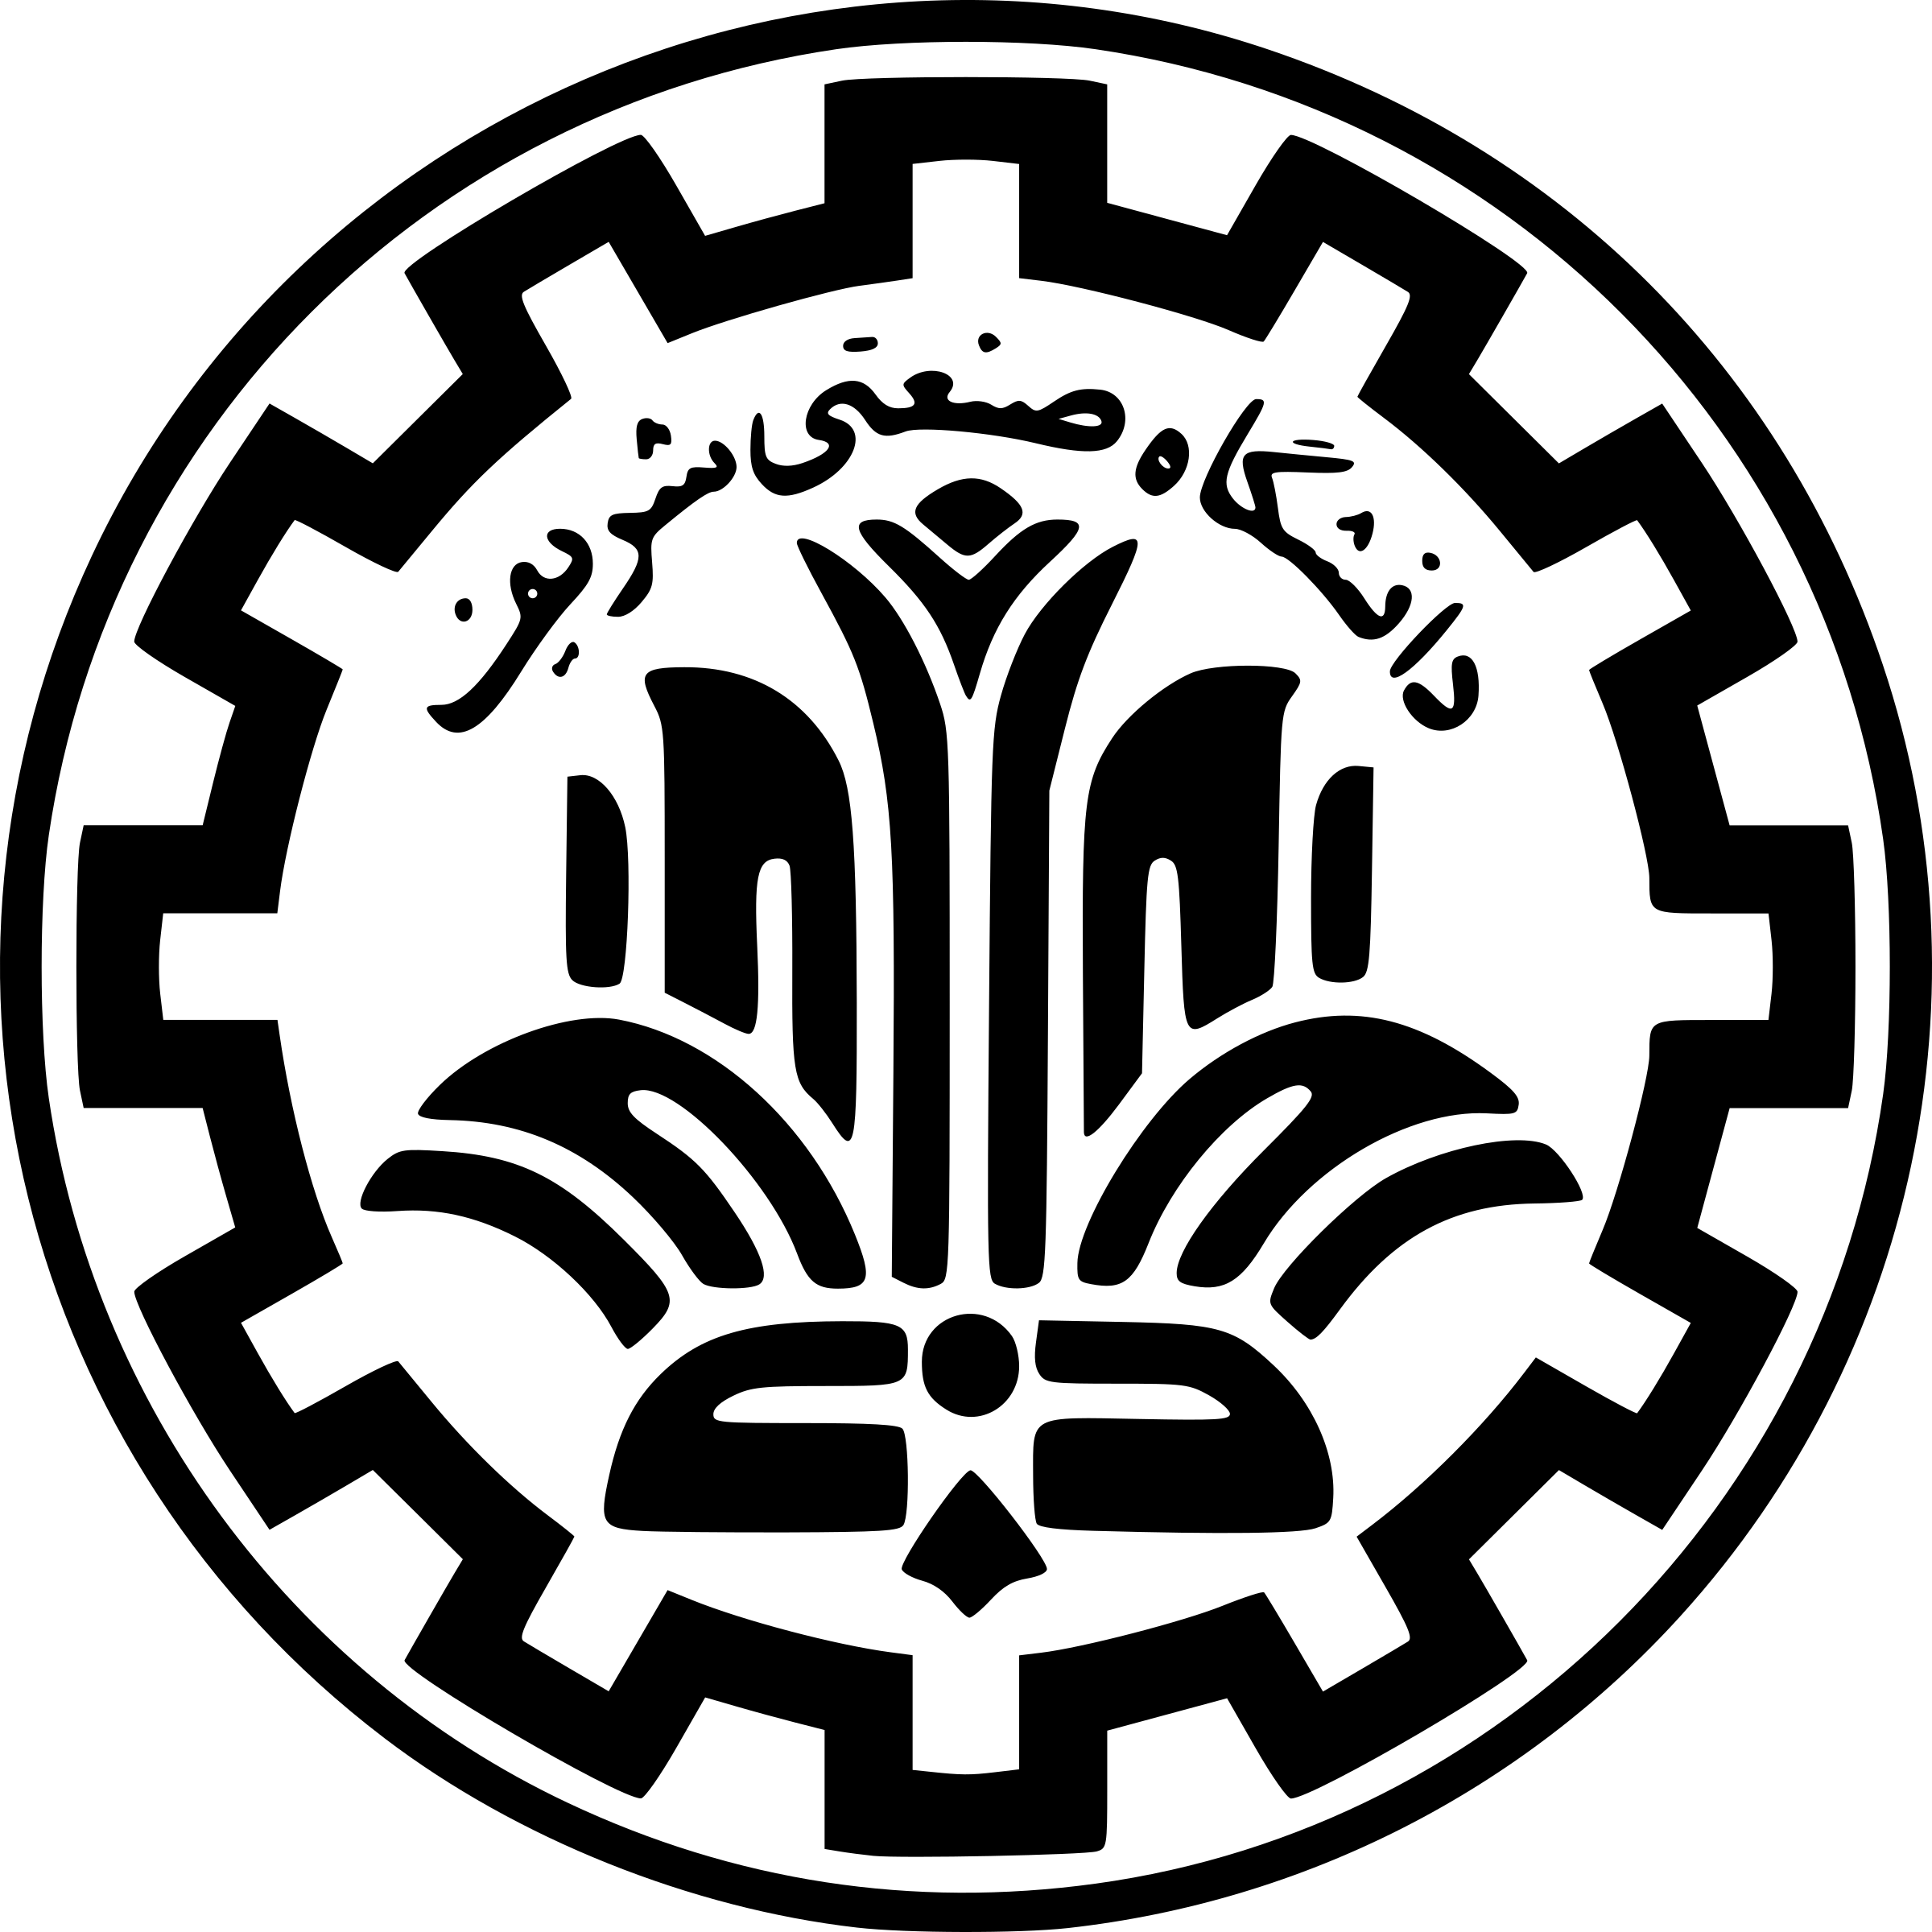
\includegraphics[width=4cm]{images/logo.png} 
    \\[1cm] 
    
    
    {\Large \textbf{گزارش آزمایش}}\\[0.3cm]
    {\Large آزمایشگاه مدار منطقی}\\[1.5cm]
    
    {\LARGE \textbf{آزمایش سوم}}\\[0.5cm]
    {\huge \textbf{شمارنده}}\\[2.5cm]
    
    
    \begin{table}[h]
        \centering
        \large
        

        اعضای گروه:\\
        \vspace{0.5cm}
        \renewcommand{\arraystretch}{1.5} 
        \begin{tabular}{|c|c|}
            \hline
            \textbf{نام و نام خانوادگی} & \textbf{شماره دانشجویی} \\
            \hline
           روناک ابوطالبی & 404105394 \\
            \hline
            حسین مرادی & 404106366 \\
            \hline
        \end{tabular}
    \end{table}
    
    \vspace{2.5cm}
    
    {\large \textbf{تاریخ تحویل: 1405/05/27}}\\[1cm]
    
    {\large \textbf{تابستان 1405}}\\[1cm]
    
    \vfill
    
\end{titlepage}

\newpage
\begin{spacing}{1.5} 
    \tableofcontents 
\end{spacing}

\newpage

\section{مقدمه و تعریف مسئله}
\leavevmode\par
\vspace{0.3cm}

\begin{spacing}{1.3}

هدف اصلی از انجام این آزمایش، آشنایی با نحوه کارکرد انواع شمارنده‌ها (Counters) است. تمامی مراحل شبیه‌سازی و پیاده‌سازی مدارهای این آزمایش باید با استفاده از نرم‌افزار پروتئوس (Proteus) انجام شود.

مسائل و خواسته‌های این آزمایش به سه بخش اصلی زیر تقسیم می‌شوند:
\end{spacing}


\subsection{شمارنده دودویی آسنکرون}
\leavevmode\par
\vspace{0.2cm}

\begin{spacing}{1.3}
در این بخش، ابتدا باید یک شمارنده بالا/پایین‌شمار آسنکرون با استفاده از چهار فلیپ‌فلاپ JK یا T طراحی شود. سپس با اعمال تغییرات لازم در مدار، امکان مقداردهی موازی نیز به آن اضافه می‌گردد. برای پیاده‌سازی این ویژگی، می‌توان از فلیپ‌فلاپ‌هایی 
استفاده کرد که دارای قابلیت Clear و Preset آسنکرون هستند.
\end{spacing}

\subsection{شمارنده دودویی سنکرون}
\leavevmode\par
\vspace{0.2cm}

\begin{spacing}{1.3}
در بخش دوم، هدف طراحی یک شمارنده سنکرون با استفاده از سه فلیپ‌فلاپ JK است که قادر باشد اعداد صفر تا هفت را سه‌تا سه‌تا بشمارد. این شمارنده دارای یک ورودی کنترلی به نام $X$ است که جهت شمارش را تعیین می‌کند؛ به این صورت که اگر $X=0$ باشد شمارش رو به پایین، و اگر $X=1$ باشد شمارش رو به بالا انجام خواهد شد.
\end{spacing}

\subsection{شمارنده BCD}
\leavevmode\par
\vspace{0.2cm}

\begin{spacing}{1.3}
در بخش نهایی، با استفاده از دو تراشه 74190 که یک شمارنده BCD با قابلیت مقداردهی اولیه و شمارش رو به بالا و پایین است، یک شمارنده برای شمارش اعداد صفر تا ۶۳ ساخته می‌شود. خروجی این شمارنده‌ها باید به نمایشگرهای هفت‌قطعه‌ای (\lr{7-Segment LED}) متصل گردد. در طراحی این بخش باید توجه شود که تا جای ممکن از به‌کارگیری مدارهای منطقی اضافه پرهیز شود.
\end{spacing}

\newpage

\section{بررسی و انتخاب روش طراحی}
\leavevmode\par
\vspace{0.3cm}

\subsection{شمارنده دودویی آسنکرون}
\leavevmode\par
\vspace{0.2cm}


\begin{spacing}{1.3}
شمارنده‌های آسنکرون\LTRfootnote{Asynchronous Counters} مدارهایی هستند که در آن‌ها پالس ساعت \lr{(Clock)} به طور همزمان به تمامی فلیپ‌فلاپ‌ها اعمال نمی‌شود؛ بلکه تنها فلیپ‌فلاپ اول پالس اصلی را دریافت کرده و سایر فلیپ‌فلاپ‌ها پالس تحریک خود را از خروجی طبقه ماقبل دریافت می‌کنند. در این مدار از  فلیپ‌فلاپ JK در طراحی استفاده شده که با اتصال ورودی‌های $J$ و $K$ یکدیگر، عملا تفاوتی با فلیپ‌فلاپ نوع \lr{T} ندارد. این ویژگی تغییر وضعیت (\lr{Toggle}) با هر لبه‌ی پالس ورودی، اساس کار شمارش در سیستم‌های دودویی است. علاوه بر این، فلیپ‌فلاپ‌های \lr{JK} معمولاً به پایه‌های کنترلی آسنکرون نظیر \lr{Preset} و \lr{Clear} مجهز هستند که پیاده‌سازی قابلیت‌هایی مانند بارگذاری موازی\LTRfootnote{Parallel Load} و مقداردهی اولیه شمارنده را بسیار ساده‌تر می‌سازد.
\end{spacing}

\subsection{شمارنده دودویی سنکرون}
\leavevmode\par
\vspace{0.2cm}

\begin{spacing}{1.3}
روش طراحی این مدار مشابه طراحی سایر مدار های سنکرون است. با استفاده از جدول حالت، حالت های بعدی را برای همه وضعیت‌های مجاز مشخص می‌کنیم و توابع ورودی‌های فلیپ‌فلاپ‌ها را با ساده سازی به کمک جدول کارنو یا روش‌های دیگر می‌سازیم.
\end{spacing}

\subsection{شمارنده BCD}
\leavevmode\par
\vspace{0.2cm}

\begin{spacing}{1.3}
در طراحی این مدار از دو تراشه 74190 استفاده می‌کنیم که هر یک مسئول کنترل یکی از رقم‌ها هستند. قطعه \lr{7-Segment} استفاده شده در این مدار خود دارای یک دیکودر\LTRfootnote{Decoder} داخلی است و عدد ورودی چهاربیتی را نمایش می‌دهد. البته عدد ورودی باید در بازه 9-0 باشد.

همچنین در طراحی این مدار از دو تراشه 74157 نیز که یک \lr{Selector/Multiplexer} است برای انجام راحت‌تر بارگذاری موازی و کنترل بازه شمارش (63-0) کمک می‌گیریم.
\end{spacing}

\section{بلوک‌دیاگرام اولیه}
\leavevmode\par
\vspace{0.3cm}

\subsection{شمارنده دودویی آسنکرون}
\leavevmode\par
\vspace{0.2cm}

\begin{center}
\begin{tikzpicture}[
    node distance=1cm and 0.8cm,
    basebox/.style={
        rectangle, draw=black, thick, rounded corners=1mm,
        minimum height=1.2cm, minimum width=1.8cm, align=center
    },
    greenbox/.style={basebox, fill=green!10},
    bluebox/.style={basebox, fill=blue!10},
    arrow/.style={-Latex, thick}
]

    \node[greenbox] (input) {ورودی‌ها \\ \lr{Clock, U/D}};
    \node[bluebox, right=of input] (logic) {منطق کنترل جهت \\ \lr{U/D Logic}};
    \node[bluebox, right=of logic] (chain) {زنجیره فلیپ‌فلاپ‌ها \\ \lr{Async FF Chain}};
    \node[greenbox, right=of chain] (out) {خروجی‌ها \\ \lr{$Q_0..Q_3$}};

    \draw[arrow] (input) -- (logic);
    \draw[arrow] (logic) -- (chain);
    \draw[arrow] (chain) -- (out);

\end{tikzpicture}
\captionof{figure}{بلوک‌دیاگرام شمارنده دودویی آسنکرون بالا/پایین‌شمار}
\label{fig:async_counter_simple}
\end{center}

\begin{center}
\begin{tikzpicture}[
    node distance=1cm and 0.8cm,
    basebox/.style={
        rectangle, draw=black, thick, rounded corners=1mm,
        minimum height=1.2cm, minimum width=1.8cm, align=center
    },
    greenbox/.style={basebox, fill=green!10},
    bluebox/.style={basebox, fill=blue!10},
    arrow/.style={-Latex, thick}
]

    \node[greenbox] (input) {ورودی‌ها \\ \lr{Data, Ld, U/D}};
    \node[bluebox, right=of input] (mode) { \lr{Mode}};
    \node[bluebox, above=of mode] (load) {\lr{Parallel Load}};
    \node[bluebox, right=of load] (preset) {\lr{Preset/Clear}};
    \node[bluebox, below=of mode] (count) {\lr{Count (U/D)}};
    \node[bluebox, right=of count] (chain) {\lr{Async FF Chain}};
    
    \node[greenbox, right=2.5cm of mode] (out) {خروجی‌ها \\ \lr{$Q_0..Q_3$}};

    \draw[arrow] (input) -- (mode);
    \draw[arrow] (mode) -- (load) node[midway, left, font=\small] {$1$};
    \draw[arrow] (mode) -- (count) node[midway, left, font=\small] {$0$};
    \draw[arrow] (load) -- (preset);
    \draw[arrow] (count) -- (chain);
    \draw[arrow] (preset) -- (out);
    \draw[arrow] (chain) -- (out);

\end{tikzpicture}
\captionof{figure}{بلوک‌دیاگرام شمارنده آسنکرون با قابلیت مقداردهی موازی}
\label{fig:async_counter_parallel}
\end{center}

\subsection{شمارنده دودویی سنکرون}
\leavevmode\par
\vspace{0.2cm}

\begin{center}
\begin{tikzpicture}[
    node distance=1.2cm and 1.2cm,
    basebox/.style={
        rectangle, draw=black, thick, rounded corners=1mm,
        minimum height=1.2cm, minimum width=2cm, align=center
    },
    greenbox/.style={basebox, fill=green!10},
    bluebox/.style={basebox, fill=blue!10},
    arrow/.style={-Latex, thick}
]

    % Nodes
    \node[greenbox] (input) {ورودی‌ها \\ \lr{Clock, $X$}};
    \node[bluebox, right=1.5cm of input] (logic) {\rl{منطق ترکیبی} \\ \lr{Next State Logic}};
    \node[bluebox, right=1.5cm of logic] (ffs) {\rl{فلیپ‌فلاپ‌های سنکرون }\\ \lr{3 $\times$ JK FFs}};
    \node[greenbox, right=1.5cm of ffs] (out) {خروجی‌ها \\ \lr{$Q_0..Q_2$}};

    % Main data flow arrows
    \draw[arrow] (input) -- (logic) node[midway, above, font=\small] {\lr{$X$}};
    \draw[arrow] (logic) -- (ffs) node[midway, above, font=\small] {\lr{J, K}};
    \draw[arrow] (ffs) -- (out) node[midway, above, font=\small] {\lr{Q}};
    
    % Clock routing (from input to FFs directly)
    \draw[arrow] (input.south) -- ++(0,-0.8) -| (ffs.south) node[near end, left, font=\small] {\lr{Clock}};
    
    % Feedback loop (Current state to Next State Logic)
    \draw[arrow] (ffs.north) -- ++(0,0.8) -| (logic.north) node[near start, above, font=\small] {Current State Feedback};

\end{tikzpicture}
\captionof{figure}{بلوک‌دیاگرام شمارنده دودویی سنکرون (با گام سه‌تایی و قابلیت تعیین جهت)}
\label{fig:sync_counter}
\end{center}


\subsection{شمارنده BCD}
\leavevmode\par
\vspace{0.2cm}


\begin{center}
\begin{tikzpicture}[
    node distance=1.5cm and 2.2cm,
    basebox/.style={
        rectangle, draw=black, thick, rounded corners=1mm,
        minimum height=1.2cm, minimum width=2.4cm, align=center
    },
    greenbox/.style={basebox, fill=green!10},
    bluebox/.style={basebox, fill=blue!10},
    orangebox/.style={basebox, fill=orange!10},
    arrow/.style={-Latex, thick}
]

    % Nodes
    \node[greenbox] (inputs) {\lr{Clock, U/D}};
    \node[greenbox, above=1.5cm of inputs] (ext) {\rl{بارگذاری کاربر}};
    
    \node[bluebox, right=2.2cm of inputs] (lsb) {\rl{شمارنده یکان} \\ \lr{74190}};
    \node[bluebox, right=2cm of lsb] (msb) {\rl{شمارنده دهگان} \\ \lr{74190}};
    
    \node[greenbox, below=1.2cm of lsb] (disp1) { \lr{7-Segment}};
    \node[greenbox, below=1.2cm of msb] (disp2) { \lr{7-Segment}};
    
    % بلوک منطق ترکیبی جدید شامل ترکیب‌کننده Load و Mux داده‌ها
    \node[orangebox, above=1.5cm of msb] (logic) {\rl{منطق ریست و لود}};

    % Main control arrows
    \draw[arrow] (inputs) -- (lsb);
    \draw[arrow] (inputs.south) -- ++(0,-0.6) -| (lsb.250) node[near end, left, font=\small] {\lr{Clock, U/D}};
    
    % Cascade arrow
    \draw[arrow] (lsb) -- (msb) node[midway, above, font=\small] {\lr{RCO}};
    
    % Outputs to display
    \draw[arrow] (lsb) -- (disp1) node[midway, left, font=\small] {};
    \draw[arrow] (msb) -- (disp2) node[midway, left, font=\small] {};
    
    % انتقال سیگنال Load و داده‌های کاربر به بلوک منطق
    \draw[arrow] (ext.east) -- (logic.west) node[midway, above, font=\small] {};

    % خطوط فیدبک برای بررسی رسیدن به عدد 64 (از لبه‌های راست و بالا)
    \draw[arrow, dashed] (msb.east) -- ++(0.5,0) |- (logic.east) node[near start, right, font=\small] {\rl{بررسی عدد 6}};
    \draw[arrow, dashed] (lsb.40) -- ++(0, 0.6) -| (logic.220) node[pos=0.3, above, font=\small] {\rl{بررسی عدد 4}}; 
    
    % خروجی‌های نهایی (فرمان Load نهایی + داده‌های Mux شده) به شمارنده‌ها
    \draw[arrow] (logic.260) -- (msb.100) node[midway, right, font=\small] {\lr{ Load  }};
    \draw[arrow] (logic.240) -- ++(0,-0.4) -| (lsb.100) node[near end, left, font=\small] {\lr{ Load }};

\end{tikzpicture}
\captionof{figure}{بلوک‌دیاگرام شمارنده BCD با قابلیت بارگذاری موازی کاربر و ریست خودکار}
\label{fig:bcd_counter_advanced}
\end{center}


\section{روند پیاده‌سازی}
\leavevmode\par
\vspace{0.3cm}

\subsection{شمارنده دودویی آسنکرون}
\leavevmode\par
\vspace{0.2cm}

\begin{spacing}{1.3}
می‌دانیم که در شمارنده آسنکرون، بیت دارای ارزش کمتر (\lr{LSB}) در هر کلاک باید تغییر کند. ابتدا سعی می‌کنیم مداری طراحی کنیم که به صورت بالارونده می‌شمارد. بنابراین ورودی \lr{Toggle} فلیپ‌فلاپ مربوط به این بیت را به ثابت یک متصل می‌کنیم. سایر بیت ها زمانی \lr{Toggle} می‌شوند که بیت سمت راست آنها از یک به صفر برود. از آنجا که فلیپ‌فلاپ های ما با لبه بالارونده کلاک کار می‌کنند، باید ورودی آنها را از $\overline{Q}$ فلیپ‌فلاپ سمت راست بگیریم تا با هربار تغییر مقدار یک فلیپ‌فلاپ از یک به صفر، فلیپ‌فلاپ سمت چپ کلاک خورده و \lr{Toggle} شود.

اگر می‌خواستیم همین مدار را به گونه‌ای طراحی کنیم که به صورت معکوس بشمارد، کافی بود کلاک فلیپ‌فلاپ‌های دیگر را معکوس کنیم، یعنی به جای $\overline{Q}$، ورودی فلیپ‌فلاپ‌های سمت چپ را به $Q$ فلیپ‌فلاپ سمت راست متصل کنیم.
حال برای طراحی مداری که به کمک ورودی‌های کنترلی \lr{Count Up} و \lr{Count Down} بتواند هم بالارونده و هم پایین رونده بشمارد، کلاک فلیپ‌فلاپ‌ها(به جز \lr{LSB}) را به جای اینکه مستقیما به $Q$ یا $\overline{Q}$ فلیپ‌فلاپ سمت راست متصل کنیم، با تابع زیر می‌سازیم:
\end{spacing}
\begin{latin}
$$C_i = D \cdot Q_{i-1} + U \cdot \overline{Q}_{i-1}$$
$$D = \text{Count Down} , U = \text{Count Up}$$
\end{latin}

\begin{spacing}{1.3}
برای اینکه در صورت برابری مقادیر \lr{Count Down} و \lr{Count Up} مدار کار نکند (حالات غیر مجاز) کلاک را با \lr{XOR} این دو ورودی \lr{AND} می‌کنیم و به کلاک فلیپ‌فلاپ اول می‌دهیم.

\vspace{0.1cm}

برای افزودن قابلیت بارگذاری موازی، ابتدا با \lr{AND} کردن $\overline{\text{COUNT}}$ و \lr{LOAD} مطمئن می‌شویم این قابلیت تنها زمانی که $\text{COUNT} = 0$ و $\text{LOAD} = 1$ فعال می‌شود. با استفاده از خروجی این گیت \lr{AND} و بیت‌های ورودی موازی، توابع ساده‌ای که به پایه‌های \lr{S} و \lr{R} فلیپ‌فلاپ‌ها متصل می‌شوند را می‌سازیم.
\end{spacing}


$$ S_i = \overline{(\text{PLOAD} \cdot P_i)}$$
$$ R_i = \overline{(\text{PLOAD} \cdot \overline{P_i)}}$$

\begin{spacing}{1.3}
دلیل استفاده از گیت‌های \lr{NAND} این است که پایه‌های \lr{R} و \lr{S} در فلیپ‌فلاپ‌های استفاده شده\\ \lr{Active Low} هستند.

از آنجا که در این مدار دو وروری مجزای \lr{Count Up} و \lr{Count Down} نداریم، با استفاده از دو گیت \lr{XOR} و \lr{AND}، سیگنال‌های مورد نیاز برای تعیین جهت شمارش را با توجه به مقدار \lr{COUNT} در حالتی که \lr{LOAD} صفر باشد می‌سازیم.
\end{spacing}

\subsection{شمارنده دودویی سنکرون}
\leavevmode\par
\vspace{0.2cm}

\begin{spacing}{1.3}
ابتدا جدول حالت مدار(جدول \ref{tab:state_table}) را رسم کرده و برای هر حالت مدار، حالت بعدی به ازای مقادیر مختلف \lr{$X$} را می‌نویسیم و وضعیت \lr{Toggle} شدن فلیپ‌فلاپ‌ها را در هر تغییر حالت یادداشت می‌کنیم.
\end{spacing}


\begin{table}[htbp]
\centering
\caption{جدول حالت شمارنده سنکرون با گام سه‌تایی}
\label{tab:state_table}
\renewcommand{\arraystretch}{1.2}
\begin{tabular}{|c|ccc|ccc|ccc|}
\hline
\multirow{2}{*}{\textbf{ورودی ($X$)}} & \multicolumn{3}{c|}{\textbf{حالت فعلی}} & \multicolumn{3}{c|}{\textbf{حالت بعدی}} & \multicolumn{3}{c|}{\textbf{ورودی فلیپ‌فلاپ‌ها}} \\ \cline{2-10} 
 & \textbf{$Q_2$} & \textbf{$Q_1$} & \textbf{$Q_0$} & \textbf{$Q_2^+$} & \textbf{$Q_1^+$} & \textbf{$Q_0^+$} & \textbf{$T_2$} & \textbf{$T_1$} & \textbf{$T_0$} \\ \hline
0 & 0 & 0 & 0 & 1 & 0 & 1 & 1 & 0 & 1 \\
0 & 0 & 0 & 1 & 1 & 1 & 0 & 1 & 1 & 1 \\
0 & 0 & 1 & 0 & 1 & 1 & 1 & 1 & 0 & 1 \\
0 & 0 & 1 & 1 & 0 & 0 & 0 & 0 & 1 & 1 \\
0 & 1 & 0 & 0 & 0 & 0 & 1 & 1 & 0 & 1 \\
0 & 1 & 0 & 1 & 0 & 1 & 0 & 1 & 1 & 1 \\
0 & 1 & 1 & 0 & 0 & 1 & 1 & 1 & 0 & 1 \\
0 & 1 & 1 & 1 & 1 & 0 & 0 & 0 & 1 & 1 \\ \hline
1 & 0 & 0 & 0 & 0 & 1 & 1 & 0 & 1 & 1 \\
1 & 0 & 0 & 1 & 1 & 0 & 0 & 1 & 0 & 1 \\
1 & 0 & 1 & 0 & 1 & 0 & 1 & 1 & 1 & 1 \\
1 & 0 & 1 & 1 & 1 & 1 & 0 & 1 & 0 & 1 \\
1 & 1 & 0 & 0 & 1 & 1 & 1 & 0 & 1 & 1 \\
1 & 1 & 0 & 1 & 0 & 0 & 0 & 1 & 0 & 1 \\
1 & 1 & 1 & 0 & 0 & 0 & 1 & 1 & 1 & 1 \\
1 & 1 & 1 & 1 & 0 & 1 & 0 & 1 & 0 & 1 \\ \hline
\end{tabular}
\end{table}

\vspace{0.5cm}

\textbf{توابع تحریک فلیپ‌فلاپ‌ها:}

با ساده‌سازی مقادیر به دست آمده برای $T_2$، $T_1$ و $T_0$، معادلات زیر به دست می‌آیند:

\begin{align*}
T_0 &= 1 \\
T_1 &= X \oplus Q_0 \\
T_2 &= \overline{T_1 \cdot \overline{Q_1 \oplus Q_0}}
\end{align*}

\textit{توجه:} از آنجا که در این طراحی از فلیپ‌فلاپ‌های JK استفاده می‌شود، پایه‌های J و K هر فلیپ‌فلاپ به هم متصل شده و معادل معادله T بالا به آن‌ها اعمال می‌گردد (یعنی $J_0=K_0=T_0$ و به همین ترتیب برای بقیه).

\subsection{شمارنده BCD}
\leavevmode\par
\vspace{0.2cm}

\begin{spacing}{1.3}
پایه های 3، 2، 6، و 7 هر دو شمارنده را به پایه‌های \lr{7-Segment} متصل می‌کنیم. این پایه‌ها خروجی تراشه 74190 به ترتیب از کم‌ارزش‌ترین بیت به پر‌ارزش‌ترین بیت هستند. همچنین پایه‌های 15، 1، 10 و 9 که ورودی‌های شمارنده برای مقداردهی اولیه هستند را به ترتیب به خروجی‌های مالتیپلکسر یعنی پایه‌های 4، 7، 9 و 12 متصل می‌کنیم.

تراشه 74157 دو گروه ورودی \lr{A} و \lr{B} دارد که با توجه به مقدار ورودی پایه شماره یک، چهاربیتی که به خروجی می‌فرستد را انتخاب می‌کند. ما در اینجا از گروه \lr{B} برای گرفتن مقدار اولیه وارد شده توسط کاربر استفاده می‌کنیم. پایه های مربوط به بیت‌های ورودی گروه \lr{A} را به گونه‌ای به مقادیر ثابت و ورودی کنترل کننده جهت شمارش متصل می‌کنیم که در صورتی که جهت شمارش رو به پایین بود مقدار این گروه برای مالتیپلکسر مسئول شمارنده دهگان شش و برای مالتیپلکسر مسئول شمارنده یکان سه باشد. در صورتی که شمارش رو به بالا باشد این مقدار برای هر دو رقم برابر صفر خواهد بود. از این ویژگی در کنترل بازه شمارش استفاده خواهیم کرد.

کلاک مدار را به کلاک شمارنده یکان متصل می‌کنیم، و خروجی \lr{RCO\LTRfootnote{Ripple Carry Output}} این شمارنده را به کلاک شمارنده دهگان وصل می‌کنیم. این خروجی هربار که رقم یکان در شمارش رو به بالا از 9 به صفر یا در شمارش رو به پایین از صفر به 9 برسد، یک سیگنال پایین-فعال‌شونده ارسال می‌کند.

پایه شماره یازده شمارنده‌ها مربوط به بارگذاری موازی است. مدار ما در هر یک از سه حالت زیر وارد حالت بارگذاری موازی(ناهمگام) می‌شود:
\end{spacing}

\vspace{-0.2cm}

\begin{itemize}
\item ورودی کنترلی \lr{P-Input} توسط کاربر به مقدار یک تنظیم شود.
\item در حالتی که شمارش رو به بالا است، به عدد 64 برسیم، در این صورت به حالت بارگاری موازی رفته و مقادیر پیش‌فرضی که برای وروری گروه \lr{A} در نظر گرفته بودیم، که در این حالت برابر با صفر است، عدد نمایش داده شده را به صفر بر می‌گرداند.
\item در حالتی که شمارش رو به پایین است، به عدد صفر برسیم، در این صورت به حالت بارگاری موازی رفته و مقادیر پیش‌فرضی که برای وروری گروه \lr{A} در نظر گرفته بودیم، که در این حالت برابر با شش و سه است، عدد نمایش داده شده را به 63 بر می‌گرداند.
\end{itemize}

\begin{spacing}{1.3}
بنابراین پایه یازده هر دو شمارنده به یک گیت \lr{NOR} متصل می‌شود که این سه شرط را بررسی می‌کند. علت استفاده از گیت \lr{NOR} این است که پایه یازده این شمارنده نیز \lr{Active-Low} می‌باشد.
پایه شماره پنج هر دو شمارنده نیز ورودی کنترلی تعیین کننده جهت شمارش است.
\end{spacing}

\newpage

\section{شماتیک نهایی مدار}
\leavevmode\par
\vspace{0.3cm}

\subsection{شمارنده دودویی آسنکرون}
\leavevmode\par
\vspace{0.2cm}

\begin{center}
    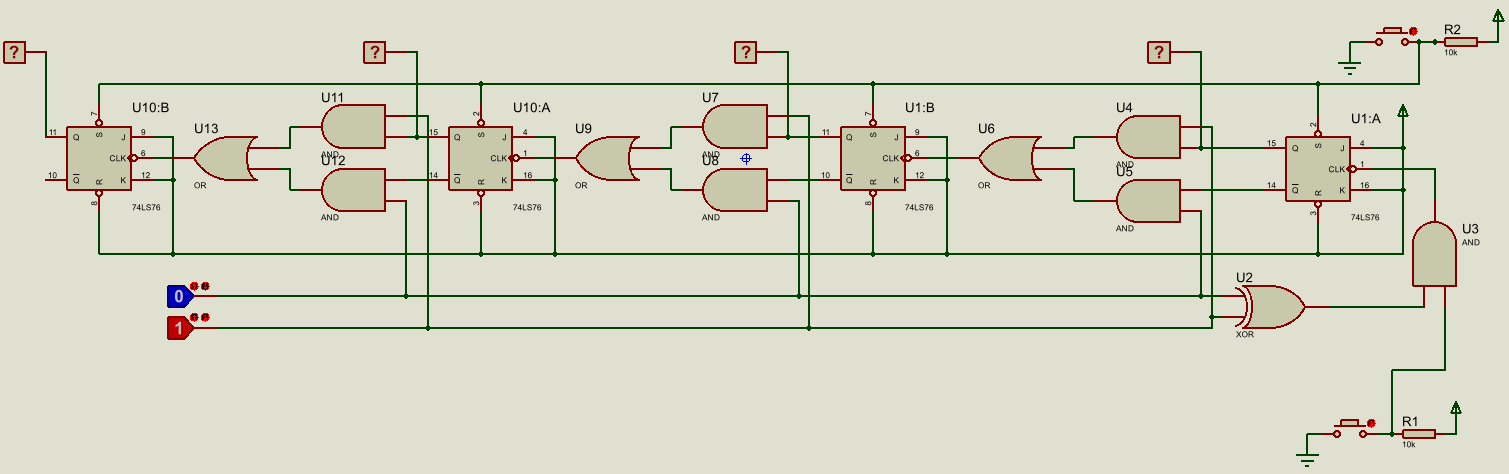
\includegraphics[width=1\textwidth]{images/1/async-simple.png}
    \captionof{figure}{شمارنده دودویی آسنکرون بالا/پایین‌شمار}
    \label{fig:async-simple}
\end{center}

\begin{center}
    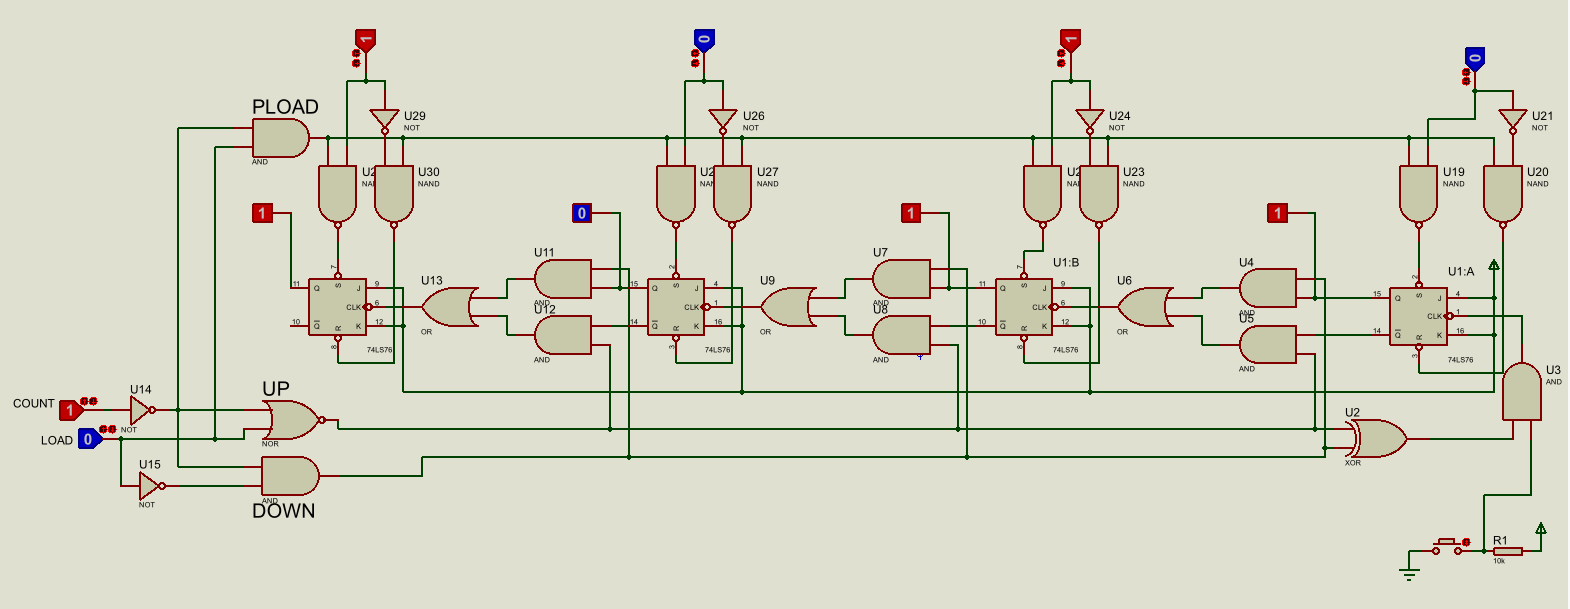
\includegraphics[width=1\textwidth]{images/1/async-pload.png}
    \captionof{figure}{شمارنده آسنکرون با قابلیت مقداردهی موازی}
    \label{fig:async-pload}
\end{center}

\subsection{شمارنده دودویی سنکرون}
\leavevmode\par
\vspace{0.2cm}

\begin{center}
    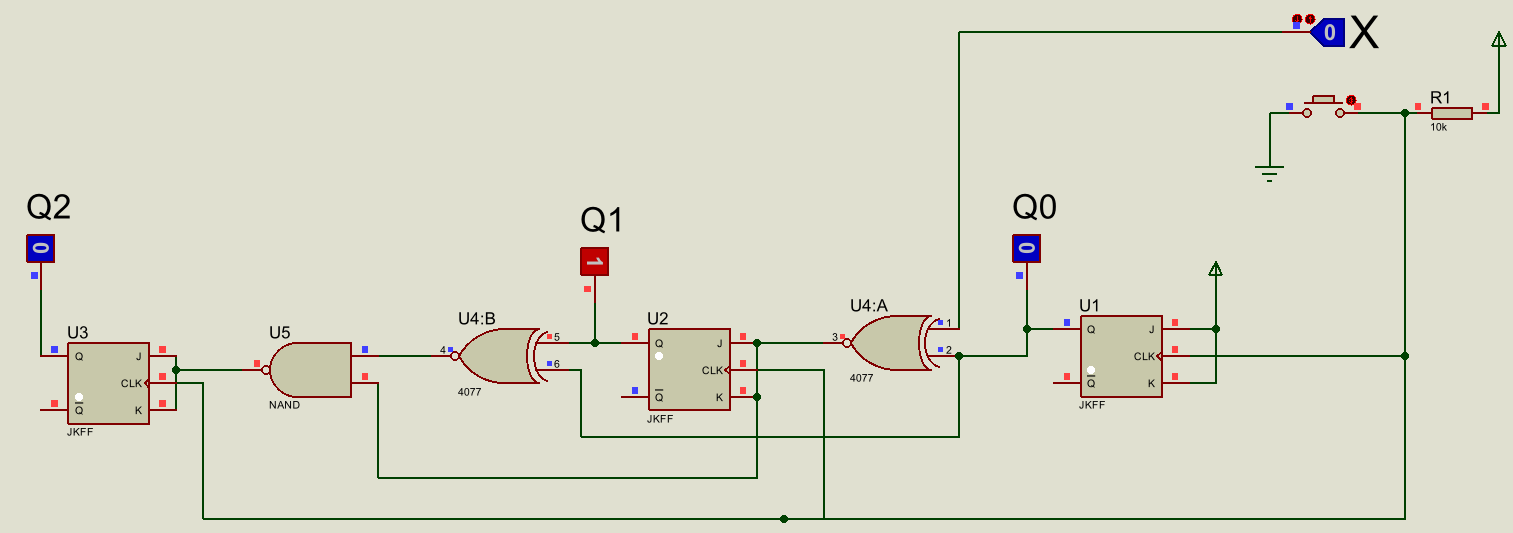
\includegraphics[width=1\textwidth]{images/2/sync-counter.png}
    \captionof{figure}{شمارنده سنکرون با گام سه‌تایی}
    \label{fig:sync-counter}
\end{center}

\subsection{شمارنده BCD}
\leavevmode\par
\vspace{0.2cm}

\begin{center}
    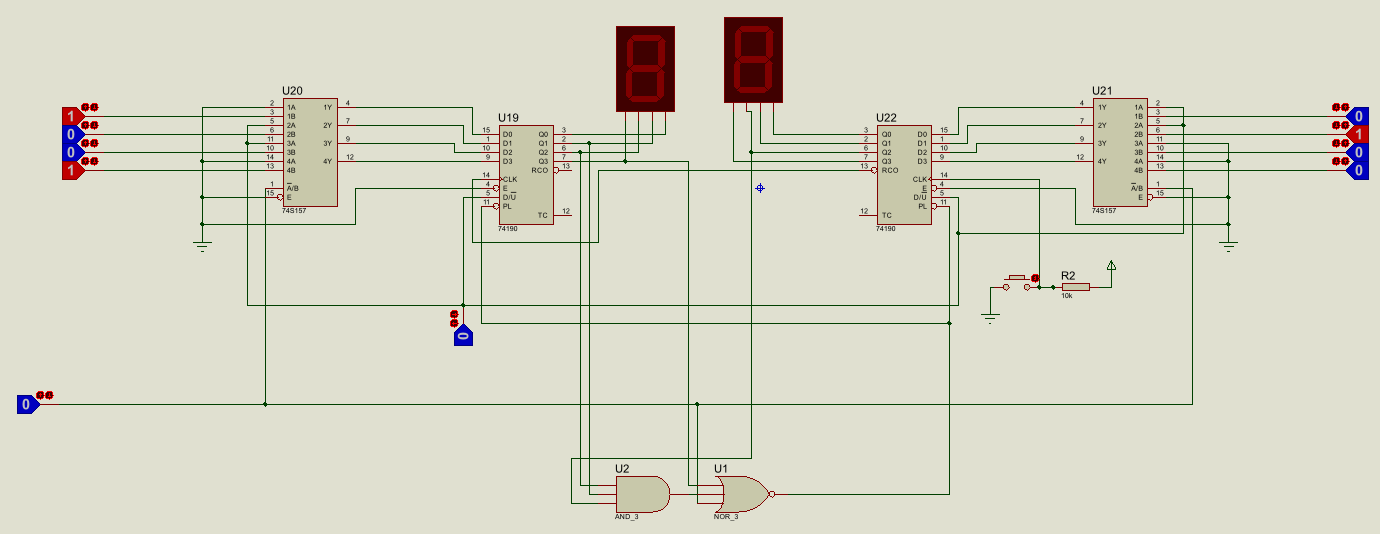
\includegraphics[width=1\textwidth]{images/3/bcd.png}
    \captionof{figure}{شمارنده \lr{BCD}}
    \label{fig:bcd}
\end{center}

\section{بررسی \lr{Test Case}ها}
\leavevmode\par
\vspace{0.3cm}

\subsection{شمارنده دودویی آسنکرون}
\leavevmode\par
\vspace{0.2cm}

شمارش رو به پایین:

\begin{center}
    
\includegraphics[width=1\textwidth]{images/1/t1.png}
    \captionof{figure}{حالت اولیه}
    \label{fig:1t1}
\end{center}

\begin{center}
    
\includegraphics[width=1\textwidth]{images/1/t2.png}
    \captionof{figure}{پس از یک کلاک}
    \label{fig:1t2}
\end{center}

شمارش رو به بالا:

\begin{center}
    
\includegraphics[width=1\textwidth]{images/1/t3.png}
    \captionof{figure}{حالت اولیه}
    \label{fig:1t3}
\end{center}

\begin{center}
    
\includegraphics[width=1\textwidth]{images/1/t4.png}
    \captionof{figure}{پس از یک کلاک}
    \label{fig:1t4}
\end{center}

قابلیت بارگذاری موازی:

\begin{center}
    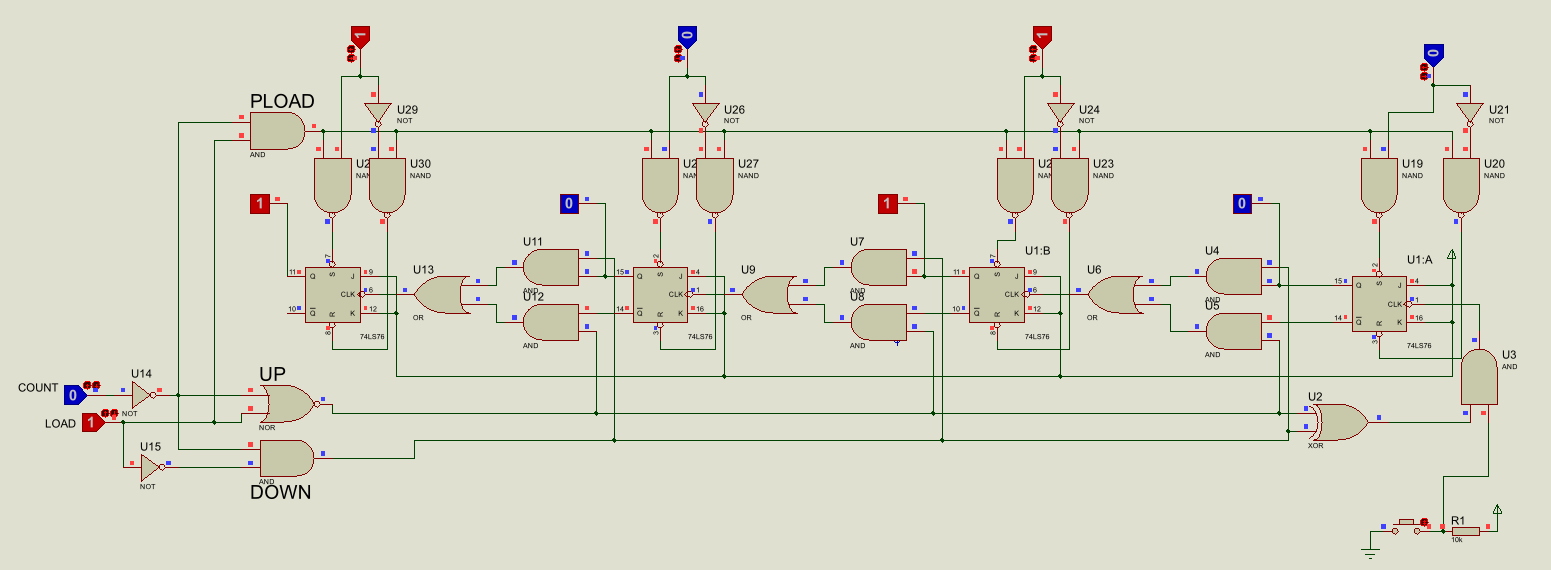
\includegraphics[width=1\textwidth]{images/1/t5.png}
    \captionof{figure}{بارگذاری موازی}
    \label{fig:1t5}
\end{center}



\subsection{شمارنده دودویی سنکرون}
\leavevmode\par
\vspace{0.2cm}

شمارش رو به بالا:

\begin{center}
    
\includegraphics[width=1\textwidth]{images/2/t1.png}
    \captionof{figure}{حالت اولیه}
    \label{fig:2t1}
\end{center}

\begin{center}
    
\includegraphics[width=1\textwidth]{images/2/t2.png}
    \captionof{figure}{پس از یک کلاک}
    \label{fig:2t2}
\end{center}

\begin{center}
    
\includegraphics[width=1\textwidth]{images/2/t3.png}
    \captionof{figure}{پس از یک کلاک دیگز}
    \label{fig:2t3}
\end{center}

شمارش رو به پایین:

\begin{center}
    
\includegraphics[width=1\textwidth]{images/2/t4.png}
    \captionof{figure}{حالت اولیه}
    \label{fig:2t4}
\end{center}

\begin{center}
    
\includegraphics[width=1\textwidth]{images/2/t5.png}
    \captionof{figure}{پس از یک کلاک}
    \label{fig:2t5}
\end{center}

\subsection{شمارنده BCD}
\leavevmode\par
\vspace{0.2cm}

بارگذاری موازی:

\begin{center}
    
\includegraphics[width=1\textwidth]{images/3/t1.png}
    \captionof{figure}{}
    \label{fig:3t1}
\end{center}

شمارش رو به بالا و عبور از 63:

\begin{center}
    
\includegraphics[width=1\textwidth]{images/3/t2.png}
    \captionof{figure}{}
    \label{fig:3t2}
\end{center}

\begin{center}
    
\includegraphics[width=1\textwidth]{images/3/t3.png}
    \captionof{figure}{}
    \label{fig:3t3}
\end{center}


\begin{center}
    
\includegraphics[width=1\textwidth]{images/3/t4.png}
    \captionof{figure}{}
    \label{fig:3t4}
\end{center}

شمارش رو به پایین و عبور از صفر:

\begin{center}
    
\includegraphics[width=1\textwidth]{images/3/t5.png}
    \captionof{figure}{}
    \label{fig:3t5}
\end{center}

\begin{center}
    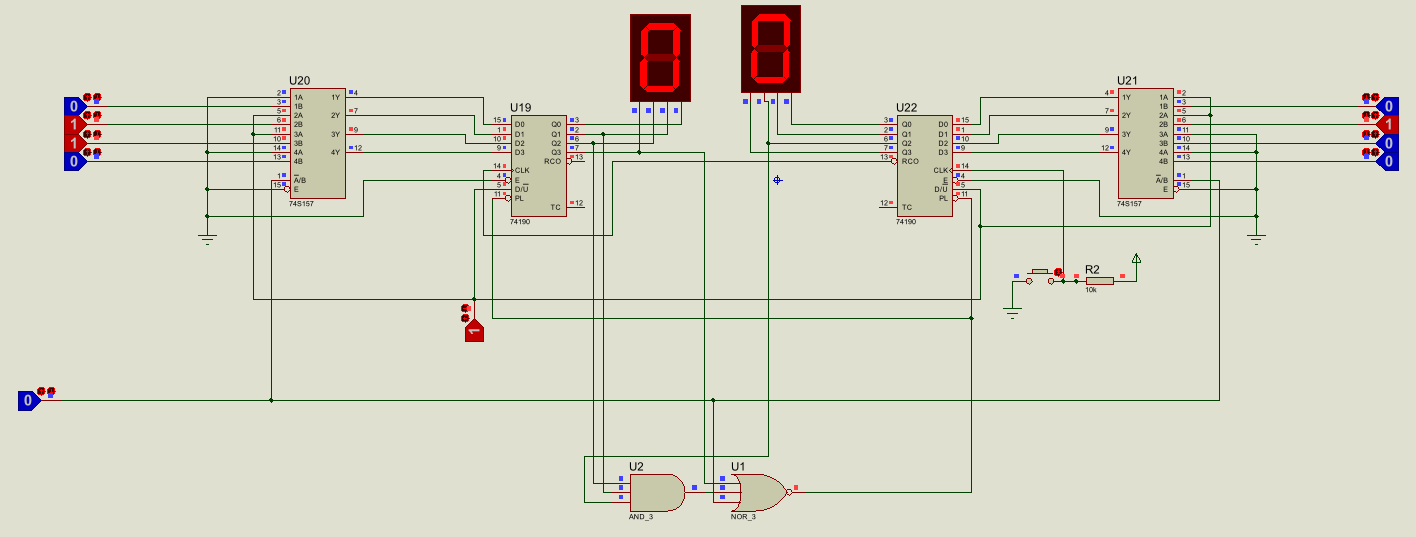
\includegraphics[width=1\textwidth]{images/3/t6.png}
    \captionof{figure}{}
    \label{fig:3t6}
\end{center}


\begin{center}
    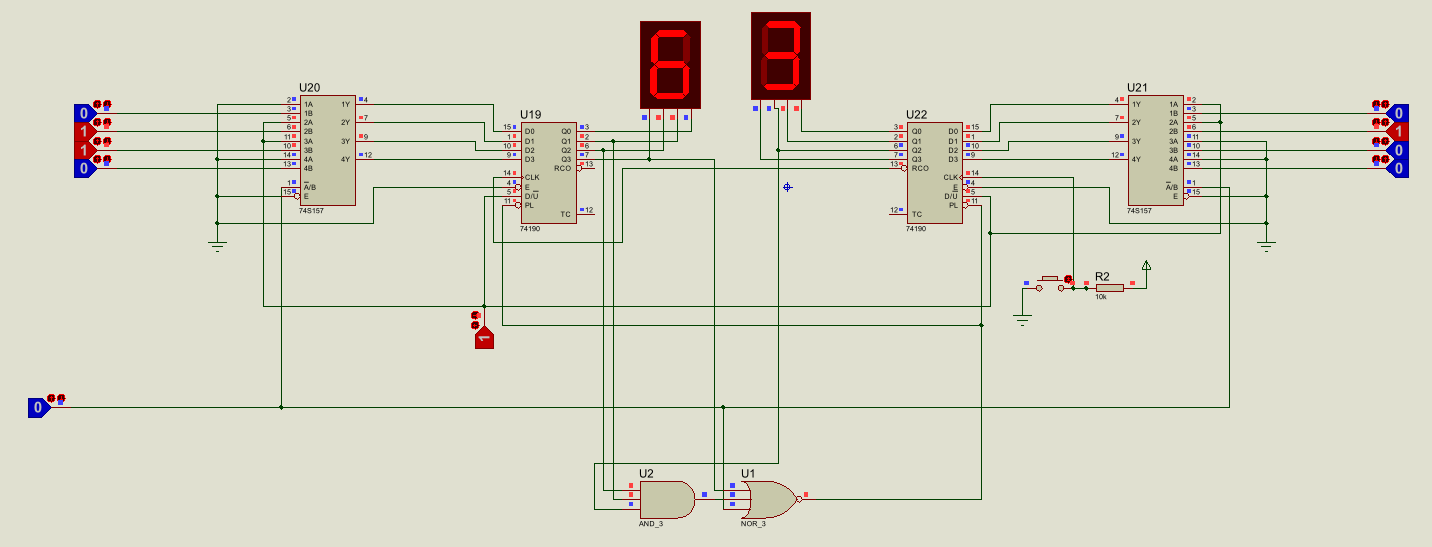
\includegraphics[width=1\textwidth]{images/3/t7.png}
    \captionof{figure}{}
    \label{fig:3t7}
\end{center}

\newpage

\section{نتیجه‌گیری}
\leavevmode\par
\vspace{0.3cm}


در این آزمایش، با اصول طراحی، تحلیل و شبیه‌سازی انواع شمارنده‌های دیجیتال آشنا شدیم و عملکرد آن‌ها را به صورت عملی در محیط نرم‌افزار پروتئوس مورد بررسی قرار دادیم. نتایج و دستاوردهای این آزمایش را می‌توان در سه بخش اصلی خلاصه کرد:

\begin{itemize}
    \item \textbf{شمارنده‌های آسنکرون (\lr{Asynchronous}):} در بخش اول، با استفاده از فلیپ‌فلاپ‌های \lr{JK} در حالت \lr{Toggle}، یک شمارنده موجی بالا/پایین‌شمار طراحی شد. همچنین با بهره‌گیری از پایه‌های آسنکرون \lr{Preset} و \lr{Clear}، قابلیت بارگذاری موازی و مقداردهی اولیه با موفقیت به مدار اضافه گردید.

    \item \textbf{شمارنده‌های سنکرون (\lr{Synchronous}):} بخش دوم، با طراحی یک شمارنده سنکرون با گام شمارش سه‌تایی، اعمال همزمان پالس ساعت به تمامی فلیپ‌فلاپ‌ها و استفاده از شبکه‌ای از گیت‌های منطقی (بر اساس جدول حالت و توابع تحریک)، نشان داد که مدارهای سنکرون از انعطاف‌پذیری و پایداری بسیار بالایی برای پیاده‌سازی الگوهای شمارش پیچیده و دلخواه برخوردارند.

    \item \textbf{شمارنده‌های \lr{BCD} و تراشه‌های آماده:} در بخش نهایی، کار با تراشه \lr{74190} به عنوان یک شمارنده مجتمع وآماده بررسی شد. با اتصال آبشاری دو تراشه از طریق پایه \lr{RCO}، یک شمارنده دو رقمی طراحی گردید. طراحی ساز و کار    توقف شمارش در 63 و همچنین دریافت وروردی موازی از کاربر از دیگر چالش های طراحی این مدار بود که با کمک گرفتن از یک مالتیپلکسر/انتخاب‌کننده برطرف شد. نمایش صحیح خروجی‌ها بر روی نمایشگرهای هفت‌قطعه‌ای (\lr{7-Segment}) نیز صحت عملکرد کلی مدار را تایید کرد.
\end{itemize}

به طور کلی، نتایج به‌دست‌آمده از شبیه‌سازی‌ها تطابق کاملی با مباحث تئوری و معادلات بولین استخراج‌شده داشت و درک عمیق‌تری از تفاوت‌ها، مزایا و کاربردهای مدارهای سنکرون و آسنکرون در سیستم‌های دیجیتال فراهم نمود.

\end{document}